% ----------------------------------------------------------------
% Report Class (This is a LaTeX2e document)  *********************
% ----------------------------------------------------------------
\documentclass[10pt]{report}
\usepackage[english]{babel}
\usepackage{amsmath,amsthm}
\usepackage{amsfonts}
\usepackage{graphicx}
\usepackage{pifont}
% THEOREMS -------------------------------------------------------
\newtheorem{thm}{Theorem}[chapter]
\newtheorem{cor}[thm]{Corollary}
\newtheorem{lem}[thm]{Lemma}
\newtheorem{prop}[thm]{Proposition}
\theoremstyle{definition}
\newtheorem{defn}[thm]{Definition}
\theoremstyle{remark}
\newtheorem{rem}[thm]{Remark}
% ----------------------------------------------------------------
\begin{document}

%\renewcommand{\thefootnote}{\fnsymbol{footnote}}

\title{\textbf{Super Blocks\footnote{the name \textbf{Tetris} is a copyright and exclusive property of Alexey Pajitnov}} \\ {\small Specification Document}}
\author{\footnotesize Human resources: \\ \scriptsize {Fakhir, Jawad}}
\maketitle

\tableofcontents

\listoffigures

\chapter{Introduction}
\section{Purpose}
The purpose of making this game is many fold:
\begin{itemize}
\item getting started with the notoriously difficult discipline of game development.
\item organizing ourselves and identifying potential problems that could arise in the development phase. (these are the problems, if ignored, can kill a startup)
\item preparing ourselves to eventually market and sell a \textbf{\underline{small scale}} game (for handheld devices like iPhone, iPad, WinPhone etc).
\item make extremely portable software. Since we are aiming for small scale games for handheld devices, it is always advisable to launch a single game simultaneously on multiple devices (iPhone, WinPhone, iPad etc). In this dynamic market we can not afford to implement a game from scratch for each of the different platforms.
    \begin{itemize}
    \item \textbf{Graphics assets portability:} keeping aspect ratio the same. In this case porting to other platforms will only be a matter of scaling up or down.
    \item \textbf{Code portability:} Reusing code as much as possible, using design patterns, using object oriented programming should be made a priority. Also the system specific code should be kept separate from the generic logic. This would slow down the speed by a tiny factor but will ensure highest portability (which is absolutely critical in small scale setup).
    \end{itemize}
\end{itemize}

\section{What is Tetris?}
You really wanna know :/ ?

\section{Why Tetris?}
This game has extremely simple graphics and logic, making it ideal to start with. We will mainly concentrate on the gameplay and logic, giving less attention to the graphics. Working prototype is expected to be made in 20 man hours whereas fully deployable and 100\% finished/polished game is expected to take 40-50 man hours.


\chapter{GUI and Main Gameplay Screen}

\section{Opening sequence}
Can be a starting movie/animation or just a splash screen. (To be decided !)

\section{Game Menu}

\begin{itemize}
\item New Game
    \begin{itemize}
    \item Survival mode
    \item Time trial mode
    \end{itemize}
\item Options
    \begin{itemize}
    \item Sound: on/off
    \item Keyboard layout (can user change these?):
        \begin{itemize}
        \item Move left: "Left arrow key"
        \item Move right: "Right arrow key"
        \item Rotate clockwise: "Up arrow key"
        \item Rotate counter clockwise: "Down arrow key"
        \item Hard drop: "Space bar"
        \item Hold piece: "Left shift"
        \item Use holding piece: "Left control"
        \end{itemize}
    \end{itemize}

\item Multiplayer
    \begin{itemize}
    \item Survival mode
    \item Time trial mode
    \end{itemize}

\item Help
\item High Score
\item Credits
\item Quit

\end{itemize}

\section{Help Screen}
To be decided !

\section{Credit Screen}
To be decided !

\section{High Score Screen}
To be decided !


\section{Main Gameplay Screen}
A random sequence of shapes called tetrominoes fall down in a $10$ tiles $\times$ $20$ tiles "well". The player can control movement of these shapes and stack them one over another. When ever a row gets completely filled (having no cavities) it is removed from the screen and everything above it shifts down by one row. The goal of the player is to survive as long as possible by stacking the shapes so as to remove maximum possible rows. Main screen is shown in figure \ref{fig:mainScreen}.

Score, time and level is displayed in the top section of the window. There are two mini panels, one at left side and one at right side.

Left panel shows "Holding" block (details in section \ref{sec:holdPiece}). Right panel shows "Next" block (details in section \ref{sec:nextPiece}).

The mini panel at the bottom left side of the main screen shows the live gameplay of another player competing with the current player.

The "nuke" icon inside the falling "I" tetromino represents special power. As soon as it hits the ground, it will clear out all of the cells in the current row (regardless if the row was already filled or not).


\begin{quote}
\ding{125}
Devices such as iPhone has a screen resolution of $320\times480$. Hence the game \textbf{aspect ratio} must be kept identical to this, i.e: $\frac{2}{3}$ or $0.666667$. This is to ensure maximum portability to other systems with minimum effort.
\ding{126}
\end{quote}

Main screen layout is yet to be decided.

\begin{figure}
\label{fig:mainScreen}
  \centering
    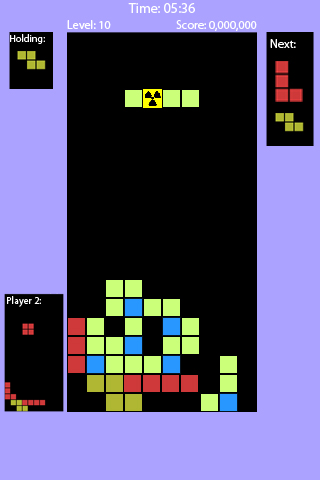
\includegraphics[width=0.5\textwidth]{mainScreen}
    \caption[Main Gameplay Screen]{The main screen. It shows almost all of the visual elements of the proposed game.}
\end{figure}

\section{Cell}
A cell/tile/block is the basic building structure of tetris. Everything is made up of cells. It can have have any shape and size but my personal preference is $20 px$ by $20 px$ solid color square or a sprite with 1 px wide "black" border as shown in figure \ref{fig:cell}.

\begin{figure}
\label{fig:cell}
  \centering
    
\includegraphics[width=0.1\textwidth]{cell}
    \caption[Tetris cell]{Tetris cell, building block of everything.}
\end{figure}


\section{Tetrominoes}
Figure \ref{fig:tetrominoes} shows the seven basic shapes in tetris. These are called Z, I, O, S, T, J, L due their resemblence with the alphabet characters. The blue cells in each tetromino represents \emph{"rotation pivot point"}. The tetrominoes will rotate about this pivot point. The color scheme is yet to be decided.

\begin{figure}
\label{fig:tetrominoes}
  \centering
    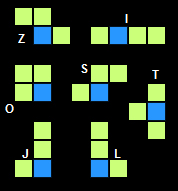
\includegraphics[width=0.3\textwidth]{tetrominoes}
    \caption[Types of tetromino]{7 different Tetrominoes. Blue cell indicates the \underline{rotation pivot} for each shape.}
\end{figure}

\chapter{Game Play}
\section{User Interaction}
\label{sec:userInteraction}
Following are some basic interaction rules:
\begin{enumerate}
\item The user can interact using ONLY the keyboard.
\item "Left" arrow key moves the tetrominoes to the left.
\item "Right" arrow key moves the tetrominoes to the right.
\item "Up" arrow key rotates the tetrominoes clockwise.
\item "Down" arrow key rotates the tetrominoes counter-clockwise. (if the piece is touching the side walls then it CANNOT be rotated.)
\item "Spacebar" will result in a "hard drop". This means that as soon as spacebar is pressed the falling tetromino will instantly hit the ground. To assist the player, a "ghost" of the falling tetromino will be constantly displayed on the ground showing the user its position if he decides to hit spacebar. The "ghost" is a vertical projection of the tetromino onto the ground, bounded by two vertical yellow lines as shown in figure \ref{fig:hardDrop}.

    After the hardDrop there will be a 1 second delay \textbf{(settling time)} to let the player adjust the piece "sideways" in order to fill cavities.
\item "Escape" pauses the game and shows the game menu. Note that the game can NOT be paused in multiplayer mode.

\end{enumerate}

\begin{figure}
\label{fig:hardDrop}
  \centering
    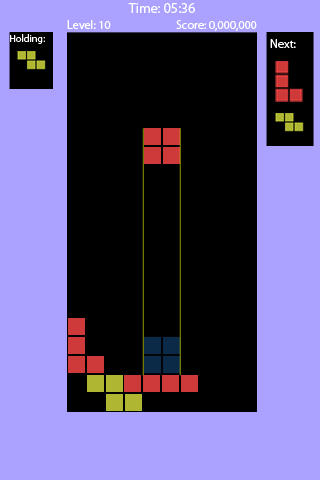
\includegraphics[width=0.6\textwidth]{hardDrop}
    \caption[Hard drop]{The ghost image (50\% opacity or alpha) (projection of the falling tetromino onto the floor to assist the user)}
\end{figure}

\section{Scoring System}
\begin{enumerate}
\item Each tetromino will be randomly spawned in the sequence having a probability $\frac{1}{7}.$
\item Score limit is capped to 9,999,999. In case if the player manages to hit this limit, the counter will stay 9,999,999 and NOT reset to zero.
\item As soon as the score upper limit is reached, current time will be stored into a seperate "score\_maxed\_at" variable and the game will continue.
\item Single clear (counted as 1 line clear) is worth 100 points.
\item Double clear (counted as 2 line clear) is worth 400 points.
\item triple clear (counted as 3 line clear) is worth 800 points.
\item Quadruple clear (counted as 4 line clear) is worth 1600 points.
\item If the tetromino was "hard-dropped" from height $h$, then a score of $h^{3}\times10$ will be added to the total score.
\item After every 10 line clears the game will advance into next level.
\item The number of levels is capped to 20.
\item There is a level multiplier:
    \begin{itemize}
    \item At the end of level $i$, current score will be multiplied by $i$.
    \end{itemize}
\item With each new level, speed of the falling tetromino will gradually increase. Speed will not increase after 20th level. (speed formula to be decided!)
\item There are no definite bounds on time limit.
\item Time bonus works as follows:
    \begin{itemize}
    \item There is a "virtual\_level" variable that constantly increments after every 10 rows cleared (in parallel to the actual level variable. The difference is that unlike actual level, there is no cap on virtual level. Virtual level is ONLY used in time bonus calculations). At the start of $i$th "virtual level", there is a pool of $i\times10000$ points. With each passing second, this pool will be decremented by 50. (This pool will become zero in exactly $\frac{10000i}{50}$ seconds).

        At the end of $i$th "virtual level", the score remaining in this pool will be added to the current score.
    \end{itemize}
\end{enumerate}

\section{Gravity}
\label{sec:gravity}
Please see the gravity section in \cite{wikitetris}.

\section{Extensions and Special Powers}
\subsection{Next Piece}
\label{sec:nextPiece}
The mini next piece window shows next 2 pieces in the sequence. The piece in the front of the queue (about to fall) will have the largest icon in the window. The 2nd piece farther away in the queue will have smaller icon. As soon as the current falling piece hits the ground and consumes its settling time, the piece in front of the "next" queue will be removed from the next window and will be placed at the top of the well. Piece in the 2nd position would be elevated to 1st position (and hence a larger icon).

\subsection{Hold Piece}
\label{sec:holdPiece}
Player has the ability to grab any falling piece and put it onto hold for future use. Current hold limit is 1 piece. As soon as the player presses "left shift" key, current falling tetromino will be deleted from the screen and saved into the "hold repository". Next piece in the que will start to fall from the very top.

If the player presses "left shift" key and the hold area already had a holding piece, then that piece would be replaced by the current falling piece.

If the player presses "left-control" key, the current falling piece would be removed from the screen and the piece in the holding area would start to fall from the top. If the holding area was already empty then left-control key has no effect.

\subsection{Nuke}
After Every 5 levels (50 rows deleted) a "nuke" will be placed in to the "pivot" of the falling tetromino with the probability $0.5$. Nuke piece is "holdable". As soon as nuke piece hits the ground and "settles" down (settling time is defined in \ref{sec:userInteraction}) the nuke will go off destroying the current row in which nuke icon was residing. At this point essential gravity computations may have to be done (section \ref{sec:gravity}).


\section{Gameplay Modes}
\label{sec:gpmodes}
To be decided !
Maybe the following:
\begin{itemize}
\item \textbf{Primary}: Survival mode (unlimited time)
\item \textbf{Secondary}: Time trial (to score high in limited time)
\end{itemize}


\section{Saving progress}
As soon as the game is over (refer to different modes in \ref{sec:gpmodes}), player score is matched across a high score table either in a local file or on a remote online server. If player score was higher than any entry in the table, that entry will be replaced by his score (user will be given a chance to input his name at this point).

\chapter{Graphics}
external assets such as animated sprites, textures created from photoshop etc. (To be decided !)

\chapter{Animation}

\section{Tetromino movement}
\textbf{\large{Please see figure \ref{fig:animation}.}}

\begin{itemize}
\item Each tetromino can only perform \underline{ONE} type of movement at a time (downward OR sideways OR rotation OR going to holding).
\item \textbf{Downwards motion}: Each tetromino will decent as follows: it will stay frozen in the current row for time $t$. After $t$ seconds it will instantaneously "jump" to the next row immediately below the current row.
\item \textbf{Sideways motion}: The piece will move to left or right columns in a very fast but smooth (non-instant) animation. Motion blur enabled.
\item \textbf{Rotation motion}: The piece rotate $\pm90^{\circ}$ non-instant but very fast and smooth motion. Motion blur enabled.
\item \textbf{Hard drop}: The piece will quickly "animate" its way down smoothly. (fast (non-instant) animation). Motion blur enabled.
\end{itemize}

\begin{figure}
\label{fig:animation}
  \centering
    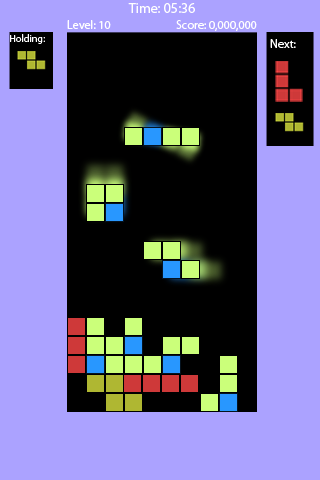
\includegraphics[width=0.6\textwidth]{animation}
    \caption[Movement Animation]{The above figure shows motion blur animation for various types of motion (drop, sideways, rotation)}
\end{figure}

\section{Holding}
\begin{itemize}
\item Suppose that the tetris is on a horizontal $XY$ plane and the player is looking vertically downwards. As soon as the player presses hold piece key, currently falling piece will glide smoothly to the holding area \underline{(motion blur is enabled)}. As it moves to the holding area its height in the vertical $Z$-axis changes. This as it moves to the holding area it gradually appears "larger" in size to the player. As soon as the piece approaches the holding area its $Z$ height will start to decrease and eventually become zero at the holding, thus appearing to be getting smaller and hence to its original size. Please see figure \ref{fig:holding}.
\end{itemize}

\begin{figure}
\label{fig:holding}
  \centering
    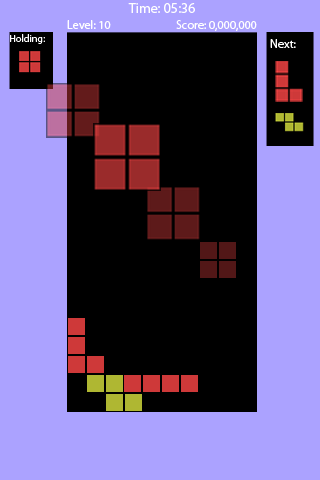
\includegraphics[width=0.6\textwidth]{holding}
    \caption[Holding Animation]{Holding animation. Notice change in height as the piece moves towards holding area \underline{(motion blur is enabled)}.}
\end{figure}

\section{Next tetromino}

\section{Tetromino touch down}

\section{Row destruction}

\section{Nuke explosion}

\chapter{Sound}
I have absolutely NO idea about this topic !

\chapter{Multiplayer}
To be decided !


\chapter{Packaging and Deploying the Game}
To be decided !

\appendix

\chapter{Resource Evaluation}

\section{Human Resources}
\begin{enumerate}
\item \textbf{Fakhir:} Responsibilities to be assigned.
\item \textbf{Jawad:} Responsibilities to be assigned.
\end{enumerate}

\section{Hardware Resources}
Following hardware is available for game development and testing:
\begin{enumerate}
\item \textbf{Fakhir:} (detailed CPUZ report can be made available upon request)
    \begin{enumerate}
    \item \textbf{Processor}: Pentium Dual-Core (E5200) 2.5 GHz
    \item \textbf{RAM}: DDR2 2.0 GB, 400Mhz, Single Channel
    \item \textbf{HDD}: 300 GB
    \item \textbf{Graphics card}: NVidia GForce 8800GT 512MB, DX10 compatible.
    \item \textbf{Printer}: Yes
    \item \textbf{Scanner}: Yes
    \item \textbf{KB/Mouse}: Yes
    \item \textbf{Camera (for capturing textures etc)}: Yes
    \item \textbf{Speaker}: Yes
    \item \textbf{Microphone}: Yes
    \item \textbf{DVD burner}: Yes
    \end{enumerate}

\item \textbf{Jawad:}
    \begin{enumerate}
    \item \textbf{N/A}:
    \end{enumerate}
\end{enumerate}


\section{Software Resources}
Following softwares are available for game development, testing and deployment: (We should really concentrate on freeware/opensource software)
\begin{enumerate}
\item \textbf{Fakhir:}
    \begin{enumerate}
    \item \textbf{OS}: Windows 7, MacOS X, Ubuntu (Vmware), Fedora core 12 (Vmware), Windows XP (Vmware),
    \item \textbf{Compiler}: Microsoft Visual Studio 2010 Ultimate, Microsoft Visual C\# 2010 Express, Cygwin, Xcode (MacOS X)
    \item \textbf{SDKs}: DX10 SDK, Nvidia DX/OpenGL SDK, iPhone SDK (MacOS X)
    \item \textbf{2D editors}: Photoshop CS5, Corel Painter 11
    \item \textbf{3D modeling}: 3D Studio Max 2010, Zbrush, Blender
    \item \textbf{Sound editors}: \underline{None}
    \item \textbf{Version control system}: \underline{None}
    \item \textbf{Communication}: TeamViewer, Skype, MSN messenger etc
    \end{enumerate}

\item \textbf{Jawad:}
    \begin{enumerate}
    \item \textbf{N/A}:
    \end{enumerate}
\end{enumerate}




\begin{thebibliography}{1}

	\bibitem{wikitetris}
	  Tetris,
	  http://en.wikipedia.org/wiki/Tetris

\end{thebibliography}


\end{document}
% ----------------------------------------------------------------
